\section{Results III: how many experts, and what drives the gate?}\label{sec:kgate}

The SMoE of \cref{sec:model} fixes $K=3$ and a three-variable gate by semantic design. A
referee is entitled to ask whether either choice is supported by the data. This section answers
with a systematic comparison: six alternative expert sets ($K=1,\dots,5$), five alternative gates,
in-sample information criteria, a parametric bootstrap of the likelihood ratio, and a score test that
screens candidate state variables from the baseline fit alone. Three theoretical points come first,
because the usual tools do not apply directly.

\subsection{Theory}

\paragraph{Experts that share a semantic group.}
Two of the larger specifications add a second intercept-only expert, which shares the empty
covariate set with the crisis expert and therefore violates \cref{ass:ident}(c). Identification
then has to come from the variance functions.

\begin{proposition}[Identification with a shared semantic group]\label{prop:ident-shared}
Let \cref{ass:ident}(a)--(b) hold and let (c) hold for every pair of experts with different
mean-covariate sets. If experts $k$ and $l$ share a covariate set, assume $\delta_{k,0}\neq\delta_{l,0}$
and adopt the labelling convention $\delta_{k,0}<\delta_{l,0}$ (expert $k$ is the calmer one). Then
$p_{\btheta}=p_{\btheta'}$ almost everywhere implies $\btheta=\btheta'$.
\end{proposition}

\noindent The proof (\cref{app:proofs}) repeats the argument for \cref{prop:ident} up to the
constant permutation $\varsigma$, which can now only exchange experts within a shared group; the
convention rules out the exchange. In practice the convention is imposed after estimation by
relabelling, and it does not affect any predictive quantity.

\paragraph{Testing $K$.}
Testing $K-1$ against $K$ experts is a boundary problem with unidentified nuisance parameters. The
null is reached either when the extra expert's gate weight vanishes ($\gamma_{K,0}\to-\infty$, so its
mean and variance parameters are not identified) or when the extra expert coincides with an
existing one (so the gate parameters separating them are not identified). In either case the
information matrix is singular at the null and the likelihood ratio has no $\chi^2$ limit; for
normal mixtures it may even diverge slowly \citep{hartigan1985failure,chen2001modified}. We therefore
use three tools that do not rely on a $\chi^2$ limit. The first is out-of-sample log score, which is
what the paper is about. The second is BIC, $-2\ell_n(\hat\btheta)+\dim(\btheta)\log n$, which is a
Laplace approximation to the log marginal likelihood \citep{schwarz1978estimating} and selects the
order of a mixture consistently under conditions given by \citet{keribin2000consistent}. The third
is the fixed-design parametric bootstrap of \citet{mclachlan1987bootstrapping}: hold the covariates
at their observed values, draw $y^\ast_t$ from the fitted null model, re-estimate both models on
$y^\ast$, and compare the observed LR statistic with the bootstrap distribution. The bootstrap
treats the covariates as fixed although they are functions of past returns; this is the standard
conditional version of the test and it is conservative when the alternative improves the fit of
the covariates' own dynamics, which the SMoE does not model.

\paragraph{Screening gate variables with a score test.}
Adding a state variable $\bm w_t\in\R^d$ to the gate changes the log-odds to
$\bm\gamma_k^\top\tilde\bz_t+\bm\psi_k^\top\bm w_t$. Under $H_0:\bm\psi=\bm 0$ the number of
experts is unchanged, all parameters stay identified, and standard theory applies. The score test
is especially convenient here because Fisher's identity \eqref{eq:score} gives the new scores in
closed form at the restricted estimate.

\begin{proposition}[LM test for omitted gate variables]\label{prop:lm-gate}
Let $\hat\btheta$ be the QMLE of the SMoE with gate covariates $\bz_t$, and let the augmented model
with gate covariates $(\bz_t,\bm w_t)$ satisfy \cref{ass:ident,ass:asym} at its pseudo-true value
$(\btheta^\ast,\bm\psi^\ast)$. The score of $\bm\psi_k$ at $(\hat\btheta,\bm0)$ is
\begin{equation}\label{eq:lm-score}
  \bm s_{\psi_k}=\sum_{t=1}^n\big(\hat\tau_{tk}-\hat\pi_{tk}\big)\,\bm w_t,\qquad k=1,\dots,K-1,
\end{equation}
the covariance between the candidate variable and the regime surprise, the gap between posterior
and prior regime probabilities. Let $\bm s$ stack all scores of the augmented model at
$(\hat\btheta,\bm0)$, partition $A$ and $B$ conformably into the $\btheta$ and $\bm\psi$ blocks, and set
$C=[-A_{\psi\theta}A_{\theta\theta}^{-1},\;I]$. Then under $H_0:\bm\psi^\ast=\bm0$
\begin{equation}\label{eq:lm}
  \mathrm{LM}=(C\bm s)^\top\big(C\hat BC^\top\big)^{-1}(C\bm s)\;\xrightarrow{d}\;\chi^2_{(K-1)d},
\end{equation}
with $\hat A,\hat B$ the Hessian and Newey--West estimators of \cref{sec:estimation}. Under local
alternatives $\bm\psi^\ast=\bm h/\sqrt n$, $\mathrm{LM}$ and the robust Wald statistic from the
augmented fit have the same non-central $\chi^2$ limit.
\end{proposition}

\noindent The test needs only the baseline fit, so a list of candidate state variables can be
screened at the cost of one estimation. It also has a direct white-box reading: a state variable
belongs in the gate if it predicts the regime surprise $\tau_{tk}-\pi_{tk}$, i.e.\ if the data assign
days to regime $k$ more (or less) often than the gate expected whenever $\bm w_t$ is high. This is a
conditional moment test in the sense of \citet{newey1985maximum} and \citet{tauchen1985diagnostic},
applied to the latent regime label. The correction $C$ matters: the restricted parameters are
estimated, and the uncorrected statistic $\bm s_\psi^\top\hat B_{\psi\psi}^{-1}\bm s_\psi$ is not
$\chi^2$ under the null.

\subsection{Design}

\Cref{tab:kg-design} lists the specifications. Along the $K$ dimension we drop either of the two
covariate experts or the crisis expert ($K=2$), add a second intercept-only ``calm'' expert, a
``premium'' expert whose mean depends on the log 22-day variance and the drawdown ($K=4$), or both
($K=5$). The premium expert gives the risk--return trade-off of \citet{french1987expected} a regime of
its own: if expected returns rise with variance in some states, its variance loading is positive.
Along the gate dimension we use volatility alone, add the log VIX of the previous US trading day
\citep{whaley2000investor,bekaert2014vix}, add the signed last return (an asymmetric gate that can
react differently to up and down days), or add all three of VIX, last return and the log one-day
range variance. The VIX enters with a one-day lag for every series, so it is known at the local
close in every time zone (\cref{app:leakage}). All specifications are estimated in the same
walk-forward on all nineteen series.

\begin{table}[t]\centering\small
\caption{Specifications compared in \cref{sec:kgate}}\label{tab:kg-design}
\begin{adjustbox}{max width=\textwidth}\begin{tabular}{llll}\toprule
Name & $K$ & Experts (mean covariates) & Gate covariates\\\midrule
Gauss-HAR & 1 & single (trend + short-horizon) & --\\
SMoE-K2tc & 2 & trend; crisis & baseline\\
SMoE-K2rc & 2 & short-horizon; crisis & baseline\\
SMoE-K2tr & 2 & trend; short-horizon & baseline\\
LSTAR & 2 & trend; short-horizon & log 22d variance\\
\textbf{SMoE} & 3 & trend; short-horizon; crisis & baseline\\
MAR & 3 & as SMoE & constant\\
SMoE-K4c & 4 & + calm (intercept only) & baseline\\
SMoE-K4p & 4 & + premium (log 22d variance, drawdown) & baseline\\
SMoE-K5 & 5 & + calm + premium & baseline\\
SMoE-Gvol & 3 & as SMoE & log 22d variance\\
SMoE-Gvix & 3 & as SMoE & baseline + log VIX$_{t-1}$\\
SMoE-Gasym & 3 & as SMoE & baseline + $r_t/\hat\sigma_t$\\
SMoE-Grich & 3 & as SMoE & baseline + VIX + $r_t/\hat\sigma_t$ + log 1d variance\\
\bottomrule\end{tabular}\end{adjustbox}
\par\smallskip\footnotesize Baseline gate: log 22-day variance, 60-day scaled momentum, drawdown
from the 250-day high.
\end{table}

\subsection{Out of sample, three experts are right}

\Cref{tab:kg-oos} and \cref{fig:kg} summarise the walk-forward comparison. Along the $K$ dimension the
baseline is best. Every $K=2$ specification is significantly worse than the SMoE in log score on four
to seven series and significantly better on one; the median loss difference is $0.28$ to $0.51$
hundredths of a nat per day. Adding experts does not help either: the calm expert ($K=4$) is never
significantly better and is worse on three series, the premium expert is better on two and worse on
five, and the five-expert model is better on two and worse on nine. The single-regime Gauss-HAR is
worse on 17 of 19
series. Out-of-sample log score therefore traces an inverted U in $K$ with its maximum at three, the
number chosen by semantic design before any data were seen. The larger models also calibrate worse:
their 1\% VaR passes the Kupiec test on 13 to 15 series, against 17 for the SMoE.

Along the gate dimension one change helps. Adding the previous day's log VIX gives the best average
rank on all four losses (log score $3.26$ against $4.79$ for the SMoE, among fourteen
specifications), a lower log score than the SMoE on 13 of 19 series (significantly lower on three and
significantly higher on one), and membership of the 10\% model confidence set on all nineteen. The gain is small: the median
improvement is $0.14$ hundredths of a nat per day. A volatility-only gate is slightly worse than the
three-variable gate (significantly on three series), the asymmetric gate that adds the signed last
return is significantly different from it on only one series, and the constant-weight MAR is
significantly worse on five
series. The largest gate (VIX, last return and one-day variance) is no better than the gate with VIX
alone.

\begin{figure}[t]\centering
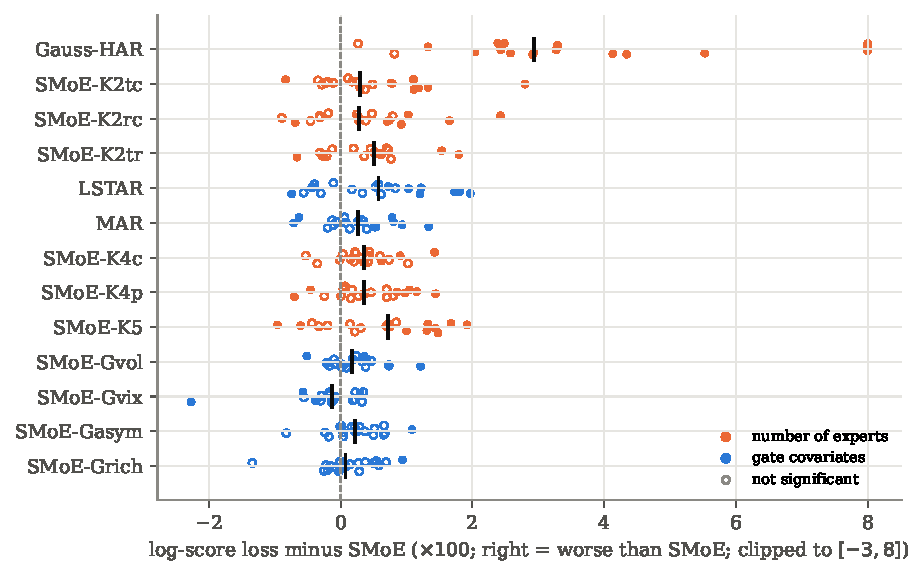
\includegraphics[width=0.92\textwidth]{../results/figures/kg_strip.pdf}
\caption{Out-of-sample log-score loss of each specification minus that of the SMoE, one point per
series (filled: DM-HLN test significant at 5\%, in either direction; vertical bars: medians). Orange:
specifications that change the experts; blue: specifications that change only the gate (LSTAR also
has $K=2$).}\label{fig:kg}
\end{figure}

\begin{table}[!htbp]\centering\footnotesize
\caption{Number of experts and gate covariates: out-of-sample comparison on 19 series (development period)}\label{tab:kg-oos}
\begin{adjustbox}{max width=\textwidth}
\begin{tabular}{lrrrrrrrrrr}
\toprule
Model & $K$ & Rank NLL & Rank CRPS & Rank QLIKE & Rank FZ5 & NLL better & NLL worse & MCS NLL & MCS QLIKE & Kupiec 1\%\\
\midrule
Gauss-HAR & 1 & 13.68 & 12.89 & 8.84 & 10.32 & 0 & 17 & 3 & 11 & 4\\
SMoE-K2tc & 2 & 7.95 & 7.53 & 9.16 & 7.32 & 1 & 7 & 15 & 14 & 17\\
SMoE-K2rc & 2 & 7.26 & 6.79 & 7.21 & 6.84 & 1 & 6 & 15 & 14 & 17\\
SMoE-K2tr & 2 & 8.42 & 8.47 & 7.74 & 6.63 & 1 & 4 & 15 & 15 & 17\\
LSTAR & 2 & 8.42 & 9.16 & 7.95 & 7.32 & 1 & 7 & 13 & 14 & 15\\
SMoE & 3 & 4.79 & 5.79 & 7.16 & 8.00 & -- & -- & 18 & 16 & 17\\
MAR & 3 & 6.74 & 5.74 & 6.89 & 7.05 & 2 & 5 & 16 & 17 & 16\\
SMoE-K4c & 4 & 7.63 & 7.16 & 7.32 & 8.47 & 0 & 3 & 18 & 17 & 14\\
SMoE-K4p & 4 & 8.05 & 8.68 & 6.21 & 8.16 & 2 & 5 & 17 & 17 & 13\\
SMoE-K5 & 5 & 9.05 & 8.68 & 7.26 & 8.68 & 2 & 9 & 17 & 17 & 15\\
SMoE-Gvol & 3 & 6.79 & 7.00 & 6.95 & 6.53 & 1 & 3 & 17 & 16 & 15\\
SMoE-Gvix & 3 & 3.26 & 5.16 & 5.84 & 5.63 & 3 & 1 & 19 & 17 & 16\\
SMoE-Gasym & 3 & 7.11 & 6.11 & 8.74 & 7.79 & 0 & 1 & 18 & 15 & 15\\
SMoE-Grich & 3 & 5.84 & 5.84 & 7.74 & 6.26 & 0 & 1 & 19 & 17 & 16\\
\bottomrule
\end{tabular}
\end{adjustbox}
\par\smallskip\begin{minipage}{\textwidth}\footnotesize
Average ranks among the 14 specifications (1 = best). NLL better/worse: series on which the specification is significantly better (one-sided DM-HLN, 5\%) or worse (two-sided, 5\%) than the SMoE in log score. MCS: series (of 19) on which the specification is in the 10\% model confidence set of the 14. Kupiec 1\%: series on which the 1\% VaR passes at 5\%.
\end{minipage}
\end{table}

\subsection{In sample, the criteria disagree}

In-sample information criteria point in opposite directions (\cref{tab:kg-bic}). Among the
specifications that differ in $K$, BIC selects two experts on 14 of 19 series and three on five; AIC
selects the five-expert model on nine series. The baseline SMoE is never the BIC choice among all fourteen
specifications, where the VIX gate is selected most often (five series). With three to five thousand
observations, BIC's penalty of $\log n\approx8$ per parameter outweighs the improvements in fit that
the walk-forward rewards, while AIC's penalty of two lets the larger models fit noise that does not
survive out of sample. Neither criterion is a reliable guide to forecasting performance here, which is
a further reason to choose $K$ by out-of-sample log score.

The parametric bootstrap makes the same point from a different angle (\cref{tab:kg-boot}). For the
CSI~300 and the S\&P~500 we test $K=1$ against $K=3$ with 199 draws and $K=3$ against $K=4$ (the
calm expert) with 99. The bootstrap null distributions are far to the right of the naive $\chi^2$
limits: for $K=1$ against $K=3$ the 95\% critical values are $39.2$ and $39.2$, against $28.9$ for a
$\chi^2_{18}$, and for $K=3$ against $K=4$ they are $24.6$ and $21.1$, against $16.9$ for a
$\chi^2_9$. This is the non-regularity described above, and a $\chi^2$ reference would over-reject.
Even against the bootstrap, both tests reject: the single regime with LR statistics of $317$ and $400$
($p=0.005$, the smallest attainable with 199 draws), and three experts in favour of four with
$62.0$ ($p=0.010$) and $43.6$ ($p=0.020$). In sample, a fourth expert is therefore supported;
out of sample, the same four-expert model is never significantly better than the SMoE and is worse
on three series. The likelihood ratio detects a fourth regime that is real in sample but does not
generalise across quarterly re-estimations.

\begin{table}[!htbp]\centering\small
\caption{Parametric bootstrap of the likelihood-ratio test for the number of experts}\label{tab:kg-boot}
\begin{adjustbox}{max width=\textwidth}
\begin{tabular}{lrrrrrr}
\toprule
Series & Test & LR & $B$ & Bootstrap 95\% crit. & Bootstrap mean & $p$\\
\midrule
CSI 300 & K1 vs K3 & 317.152 & 199 & 39.225 & 27.129 & 0.005\\
CSI 300 & K3 vs K4 & 62.018 & 99 & 24.568 & 14.494 & 0.010\\
S\&P 500 & K1 vs K3 & 399.651 & 199 & 39.186 & 25.977 & 0.005\\
S\&P 500 & K3 vs K4 & 43.622 & 99 & 21.111 & 14.010 & 0.020\\
\bottomrule
\end{tabular}
\end{adjustbox}
\par\smallskip\begin{minipage}{\textwidth}\footnotesize
Fixed-design parametric bootstrap \citep{mclachlan1987bootstrapping}: $y^\ast$ drawn from the fitted null model at the observed covariates; both models re-estimated on every draw (best of a warm start and two random starts). $p=(1+\#\{LR^\ast\ge LR\})/(1+B)$. The observed LR uses the same estimation procedure as the draws; the four-start fit of \cref{tab:csi300_lik} gives a slightly larger LR for the CSI 300 ($K=1$ against $K=3$).
\end{minipage}
\end{table}

\begin{table}[!htbp]\centering\footnotesize
\caption{In-sample model selection by BIC (development sample)}\label{tab:kg-bic}
\begin{adjustbox}{max width=\textwidth}
\begin{tabular}{lrrr}
\toprule
Asset & BIC-best (all 14) & BIC-best $K$-spec. & $\Delta$BIC SMoE\\
\midrule
SHFE gold futures & SMoE-Gvix & SMoE-K2rc & 107.3\\
Bitcoin & MAR & SMoE & 24.0\\
ChiNext & LSTAR & SMoE-K2rc & 37.9\\
WTI crude futures & SMoE-K2rc & SMoE-K2rc & 53.4\\
CSI 300 & SMoE-Gasym & SMoE-K2tc & 46.1\\
CSI 500 & SMoE-Gvol & SMoE & 13.9\\
SHFE copper futures & SMoE-Gvix & SMoE-K2tr & 10.6\\
DAX & SMoE-Gasym & SMoE-K2tr & 27.0\\
CSI 300 ETF (510300) & LSTAR & SMoE-K2tc & 50.7\\
FTSE 100 & SMoE-Grich & SMoE-K2tc & 35.3\\
COMEX gold futures & SMoE-Gvix & SMoE-K2tc & 20.5\\
Hang Seng & SMoE-K2rc & SMoE-K2rc & 15.5\\
CSI 300 futures (IF) & LSTAR & SMoE-K2rc & 60.3\\
DCE soybean meal futures & SMoE-Gvol & SMoE & 26.0\\
Nikkei 225 & SMoE-Gvix & SMoE & 23.7\\
Nasdaq 100 & SMoE-Grich & SMoE-K2rc & 45.6\\
S\&P 500 & SMoE-Gvix & SMoE & 40.4\\
SSE 50 & LSTAR & SMoE-K2tc & 45.9\\
US 10y T-note futures & SMoE-K2rc & SMoE-K2rc & 63.9\\
\bottomrule
\end{tabular}
\end{adjustbox}
\par\smallskip\begin{minipage}{\textwidth}\footnotesize
$\Delta$BIC SMoE: BIC of the baseline SMoE minus the smallest BIC (0 when the SMoE is selected).
\end{minipage}
\end{table}

\subsection{Which state variables belong in the gate?}

\Cref{tab:kg-lm} screens three candidates with the score test of \cref{prop:lm-gate}, computed from
the baseline fit alone. The VIX is rejected as irrelevant on 11 of 19 series, the signed last return
on six and the one-day variance on two. The robust Wald test from the augmented VIX fit rejects on
twelve, and the two statistics are of the same size series by series (for the S\&P~500, $37.6$ and
$46.3$ with two degrees of freedom; for SHFE gold, $36.8$ and $49.1$), as the proposition predicts
when the effect is real.

The VIX result is geographically structured. By the robust Wald test at 5\%, the US fear gauge
enters the gate of all five developed equity indices, the Hang Seng, both gold contracts, WTI crude
and soybean meal, but not that of the CSI~300 ($p=0.06$), the CSI~500, ChiNext, the IF futures,
copper, the T-note or Bitcoin. Among the A-share series only the SSE~50 and, marginally, the CSI~300
ETF ($p=0.037$, on a sample that starts in 2012) respond.
 In the developed equity indices the sign is uniform: at a given level of the index's
own 22-day variance, a higher VIX moves weight from the crisis expert to the two covariate experts
($z$ between $1.8$ and $6.0$). The VIX is forward-looking while the range-based state is not, so
conditional on recent realised variance a high VIX appears to signal risk that the trend and
short-horizon regimes, with their own variance dynamics, can carry. For the A-share market, the
absence of a VIX effect is consistent with its partial segmentation from global risk appetite. For
the CSI~300 the score test instead flags the most recent day: the one-day variance ($p=0.004$) and the
signed last return ($p=0.033$) are both rejected as irrelevant, so regime weights in the Chinese
index respond to yesterday's move as well as to the 22-day variance.

The premium expert does not find a risk--return trade-off. Its loading on the log 22-day variance is
positive and significant only for the CSI~500 and WTI and negative and significant for the CSI~300
and the SSE~50. Its loading on the drawdown state, by contrast, is negative and significant on seven
series (four Chinese equity indices, the FTSE, SHFE gold and the T-note). Because the drawdown state
$\log(P_t/\max_{j<250}P_{t-j})$ is non-positive, a negative loading means a higher expected return
deep in a drawdown. The fourth expert, given the chance, describes rebounds after large losses rather
than compensation for variance.

\begin{table}[!htbp]\centering\footnotesize
\caption{Screening gate variables: robust LM $p$-values from the baseline fit (\cref{prop:lm-gate}), development sample}\label{tab:kg-lm}
\begin{adjustbox}{max width=\textwidth}
\begin{tabular}{lrrrrrr}
\toprule
Asset & LM: VIX & LM: return & LM: 1d var. & LM: all three & Wald VIX $p$ & premium: $\beta_{\mathrm{lv22}}$ ($z$)\\
\midrule
CSI 300 & 0.083 & 0.033 & 0.004 & 0.003 & 0.060 & -0.950 (-2.8)\\
CSI 500 & 0.512 & 0.224 & 0.039 & 0.005 & 0.252 & 0.485 (4.6)\\
SSE 50 & 0.003 & 0.018 & 0.853 & 0.000 & 0.000 & -0.890 (-2.0)\\
ChiNext & 0.385 & 0.822 & 0.493 & 0.739 & 0.421 & 0.351 (1.2)\\
S\&P 500 & 0.000 & 0.081 & 0.205 & 0.000 & 0.000 & -0.576 (-0.2)\\
Nasdaq 100 & 0.000 & 0.000 & 0.957 & 0.000 & 0.000 & 0.010 (0.3)\\
Hang Seng & 0.009 & 0.337 & 0.141 & 0.010 & 0.001 & -0.136 (-0.7)\\
Nikkei 225 & 0.000 & 0.013 & 0.508 & 0.000 & 0.000 & 0.154 (0.5)\\
DAX & 0.027 & 0.002 & 0.377 & 0.004 & 0.017 & 0.290 (0.4)\\
FTSE 100 & 0.000 & 0.000 & 0.070 & 0.000 & 0.000 & 0.143 (1.1)\\
CSI 300 futures (IF) & 0.181 & 0.167 & 0.738 & 0.236 & 0.074 & 0.014 (0.1)\\
SHFE gold futures & 0.000 & 0.464 & 0.840 & 0.000 & 0.000 & -0.072 (-1.6)\\
SHFE copper futures & 0.189 & 0.139 & 0.191 & 0.120 & 0.051 & 0.067 (0.9)\\
DCE soybean meal futures & 0.001 & 0.233 & 0.708 & 0.004 & 0.000 & 0.059 (1.0)\\
WTI crude futures & 0.008 & 0.274 & 0.709 & 0.066 & 0.040 & 0.284 (2.3)\\
COMEX gold futures & 0.000 & 0.510 & 0.328 & 0.000 & 0.000 & 0.040 (0.5)\\
US 10y T-note futures & 0.385 & 0.171 & 0.565 & 0.235 & 0.165 & 0.103 (1.2)\\
Bitcoin & 0.510 & 0.963 & 0.154 & 0.460 & 0.587 & 0.110 (0.6)\\
CSI 300 ETF (510300) & 0.052 & 0.069 & 0.529 & 0.056 & 0.037 & -0.329 (-1.1)\\
\bottomrule
\end{tabular}
\end{adjustbox}
\par\smallskip\begin{minipage}{\textwidth}\footnotesize
LM: $p$-value of the score test that the candidate is absent from the gate, computed from the baseline SMoE alone ($2d$ df). Wald VIX $p$: robust Wald test of the same hypothesis for VIX from the augmented fit (SMoE-Gvix). Premium: standardised loading of the premium expert's mean on log 22-day variance in SMoE-K4p, with robust $z$-statistic.
\end{minipage}
\end{table}

\paragraph{Summary.} Three experts are supported out of sample. In sample, BIC prefers fewer and the
bootstrapped likelihood ratio prefers more, and neither choice forecasts better. The three-variable gate is a reasonable default, and the VIX is the only
addition that both passes the score test on most series and improves out-of-sample forecasts. Because
we made these comparisons on the development sample after the main specification was fixed, the
lockbox results of \cref{sec:lockbox} still refer to the original SMoE.
